\chapter{Used Technologies}
\label{chapter:ConfTechnology}
Before the problem can be explained an introduction into the technologies in question
and the terminology that is used in the rest of this document is in order. This should
only serve as a brief outline since a full explanation goes beyond the scope of this
thesis.

\section{Eclipse}
\label{section:ConfTechEclipse}
\index{Eclipse}
Since the \ac{KIELER} project and thus the Execution Manager is build upon the 
Eclipse framework a short introduction into Eclipse is necessary.

The basic function of Eclipse is as \textit{the} Java \ac{IDE}. It provides
a host of facilities that makes it easier for the user to create their own Java applications.
A few examples for these facilities are:
\begin{itemize}
 \item Syntax highlighting to make the source code easier to read.
 \item Automatic completion of partial commands to ensure correctness
and make it easier to write code.
 \item Content assist to create better code and remove errors.
 \item Several wizards for class creation and other tasks.
\end{itemize}

However since Eclipse is an open-source project there are also plug-ins for variety of
other things. For example the language isn't limited to Java. There are also plug-ins
for C++, Latex, Visual Basic and several other programming languages.

Through the use of different modeling framework Eclipse can also be used as an \ac{IDE}
for \ac{IDE}s. The best description for Eclipse is: ``an IDE for anything, and nothing in particular'' \cite{eclipseOverview}.

\begin{figure}
  \centering
  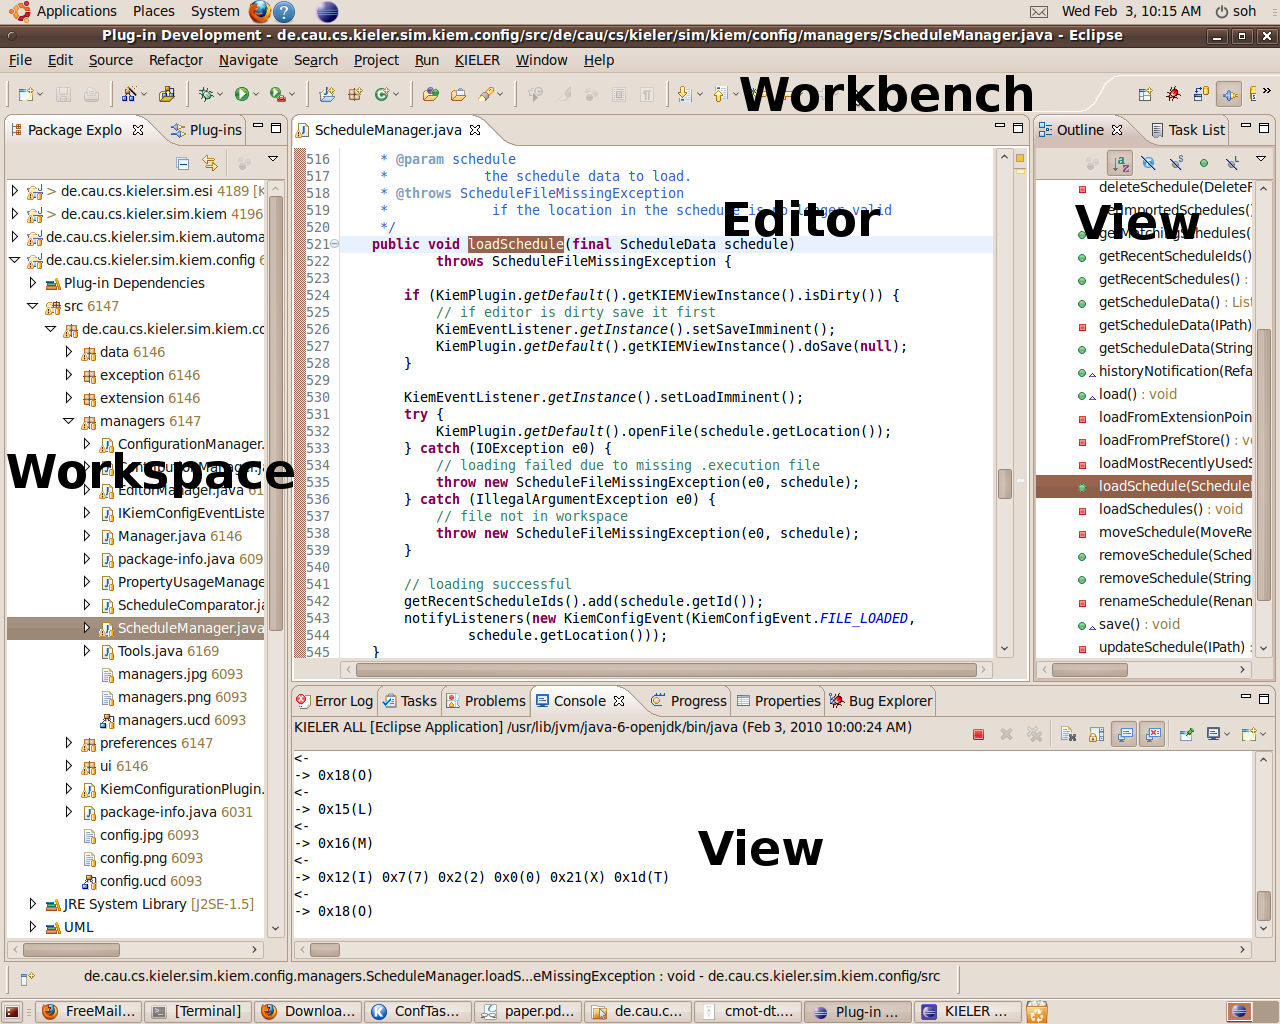
\includegraphics[scale=.3]{EclipseScreen.png}
  \caption[The Eclipse workbench window]%
  {The Eclipse workbench window\protect}
  \label{fig:EclipseScreen}
\end{figure}
The terminology used for the different basic parts of Eclipse can be illustrated based on Figure
\ref{fig:EclipseScreen}:
\begin{description}
 \item The main window of Eclipse is called the \textit{workbench}. The workbench consists of the 
different editors and views.
 \item The files that the user operates on are located in the Eclipse \textit{workspace}. 
 \item An \textit{editor} is a component that allows the user to display, enter and modify information.
Editors are used to modify a specific file type. There can usually be multiple instances of the same editor.
An example for an editor would be the Java editor which is used to create and edit Java source files.
 \item An Eclipse \textit{view} is the other component located on the workbench. Views are only used to
display content that was created elsewhere. Unlike editors there is usually only one instance of any view.
One of the views shown in the figure is the class outline view. It shows all methods and attributes of the 
Java class in the currently active editor.
\end{description}


For additional information about eclipse see the official Eclipse website\footnote{www.eclipse.org} or literature \cite{eclipsePlugins}.


\subsection{Plug-ins}
\label{section:ConfTechPlugins}
\index{Plug-in}
The building blocks of any Eclipse application are the so called \textit{plug-ins}. They
consist of any number of Java classes and additional meta information. The Java classes
describe the behavior of the plug-in and define its \ac{API}. The meta information is not written
in Java but uses an \ac{XML} notation instead. The meta information contains the following
information:
\begin{itemize}
 \item What other plug-ins does the plug-in depend on. This information is necessary to determine
which other plug-ins have to be loaded or when to refuse loading the plug-in because of missing
dependencies.
 \item What \textit{extension points} does the plug-in offer. These are part of the \ac{API} and
will be described below.
 \item What functionality does it add to the plug-ins which it extends.
\end{itemize}

Plug-ins encapsulate their internal behavior and can be accessed through the \ac{API} and the 
\textit{extension points}. They provide a specific functionality that can be reused as long as
the dependencies are met. As such an Eclipse application consists of a mosaic of different
plug-ins that can be exchanged at will.

Eclipse can not only be used to create plug-ins that can be used in an Eclipse
instance but can also compile a set of plug-ins into a standalone application - the so
called \ac{RCA}. This \ac{RCA} contains a minimal set of plug-ins to provide the Eclipse
look-and-feel and the plug-ins created by the user.

\subsubsection{Extension Point Mechanism}
\label{section:ConfTechExtension}
\index{Extension point}
The extension point mechanism is one of the key features of plug-in development in Eclipse.
It extends the \ac{API} provided by the public methods of the different Java classes inside
the plug-in. An extension point definition consists of a tree of different configuration elements.
Each configuration element has different attributes some of which can be optional while other
are mandatory. These attributes can be anything from a String, a file to a Java class that has
to extend one class and implement a specific interface.

A plug-in that wants to add their functionality to an already existing plug-in
through the use of an extension point has to provide the mandatory attributes defined in the 
specifications.

Eclipse itself already provides many extension points to extend the functionality of the workbench.
For example, if a plug-in wants to add a new editor to the workbench it has to extend the 
\textit{org.eclipse.ui.editors} extension point. It then has to provide an identifier and a name
as well as a class that implements the \textit{org.eclipse.ui.IEditorPart} interface. It can also specify an
icon and a file extension for files which should be opened with the new editor.

When an Eclipse application is started with this plug-in Eclipse will automatically make sure that the new editor
can be used to open the specified file type. The programmer only has to concern himself with the area of the editor
itself without worrying about it being added at all the necessary places inside the Eclipse architecture.

\subsection{Preference Pages}
\label{section:TechPreferencePage}
\index{Preference Page}
A special example of plug-in usage within the Eclipse framework itself is the 

\textit{org.eclipse.ui.preferencePage} plug-in. 
It is used to create new preference pages at a specific location inside the
normal tree of preference pages accessible through Window->Preferences.
The programmer only has to take care of the contents of the actual page and not worry
about additional buttons or integrating it into the PreferenceDialog.

\subsubsection{Preference Store}
\label{section:TechPreferenceStore}
Closely coupled with the preference pages is the Eclipse preference store. It is
basically a text file for each plug-in where the plug-in can deposit simple Strings
under a given key to ensure that information is kept between execution runs.